Az előző fejezetben láthattuk, milyen komponensekből épül fel a videóadat.
A következő fejezet azt taglalja, hogy az eddig tárgyalt komponensekből hogyan állnak elő a különböző analóg, valamint digitális videoformátumok, illetve ezen formátumok paraméterválasztásának kérdéseivel foglalkozik.
Láthatjuk, milyen irányelvek mentén került megválasztásra az egyes formátumok képmérete, térbeli felbontása (pixelszáma), képfrissítési frekvenciája. 
Emellett láthatjuk, hogy immár konkrét paraméterek mellett hogyan épül fel az analóg és digitális videójel.

\section{SD formátumok}

Elsőként a korai, normál felbontású NTSC és PAL analóg televíziós rendszerek képformátumát és paramétereinek megválasztását tárgyaljuk.
Bár ezen analóg rendszerek már csak elvétve vannak használatban világszerte---Magyarországon például több éves digitális átállásra való előkészülés után 2013-ban szűnt meg az analóg műsorszórás---, mégis fontos tárgyalni főbb jellemzőit.
Ennek oka történelmi jelentőségük mellett az, hogy a jelenlegi digitális műsorszórásban (a HD adás mellett) legelterjedtebb \textbf{normál felbontású (Standard Definition, SD)} digitális formátumokat közvetlenül az NTSC és PAL videojelek digitalizálásával kapjuk meg.\footnote{Pontosabban az NTSC és PAL kompozit jeleket alkotó chroma és luma komponensek digitalizálásával.}

\paragraph{Képarány és képméret:\\}
Elsőként fontos leszögezni, mekkora képméretre kell optimális formátum-paramétereket választani.
Az \ref{sec:HVS} fejezetben látható volt, hogy az emberi szemben a színlátás helye a sárgafolt, ezen belül is az éleslátásért a látógödörben (fovea centralis) elhelyezkedő receptorok felelnek.
A látógödör mérete alapján az éleslátásunk a teljes $\approx200$ fokos látószögünkből kb. 10-15 fokot fed le a horizontális irányban.\footnote{http://hyperphysics.phy-astr.gsu.edu/hbase/vision/retina.html}
A normál felbontású televíziós szabvány megalkotása során a cél ezen fő látószög tartalommal való kitöltése volt, vagyis a normál felbontású televízió kb. a látótérből 10 fokot kell, hogy kitöltsön (azaz a periférikus látásnak a képalkotásban nem volt szerepe).
Természetesen a konkrét képméret ezek után a nézőtávolság függvénye.
Adott pixelméret/sortávolság mellett az optimális nézőtávolság megválasztásával a későbbiekben foglalkozunk.

A kép mérete mellett fontos térbeli jellemző a kijelző horizontális és vertikális dimenziójának aránya, azaz az ún. \textbf{képarány}.
Az SD formátum alapjául szolgáló NTSC szabvány létrehozása az 1940-es évekig nyúlik vissza, és kidolgozása során nyilvánvaló törekvés volt a korabeli mozifilmek megjelenítésével való kompatibilitás biztosítása.
A mozi korai korszaka, így a teljes némafilm korszak (az anamorf lencsék megjelenése előtt) kizárólag 4:3 képarányt alkalmazott, azaz a horizontális és vertikális képhosszak aránya $1.3\dot{3}$ volt\footnote{A 4:3 képarány létrejötte egészen Thomas Alva Edison munkájáig vezethető vissza, aki az általa használt 35 mm széles filmen egy képkockát 4 perforációnyi magasságúra (19 mm) definiált. 
A perforációk közötti kihasználható szélességből (25.375 mm) így a hasznos terület épp 4:3-hoz képarányúra adódik. 
A 35 mm-es filmen 4 perforációnyi képméretet 1909-ben fogadták el általános szabványnak ("4-perf negative pulldown"), lehetővé téve a szabványos mozikamerák, mozigépek és így a mozi térhódítását.}.
Habár az 50-es években megjelentek az első szélesvásznú mozis formátumok, az NTSC szabvány ezt a 4:3 képarányt fogadta el a televízió szabványos képarányának.
%TODO anamorphic lenses?
% Forrás: https://www.shutterstock.com/blog/4-3-aspect-ratio
% https://www.cinematographers.nl/FORMATS1.html

\paragraph{Képfrissítési frekvencia:\\}

Következő kérdésként vizsgáljuk a mozgókép temporális mintavételi frekvenciájának, azaz a másodpercenként felvillantott képelemek számának megválasztási szempontjait.
A továbbiakban ezt a frekvenciát \textbf{képfrissítési frekvenciának} nevezzük.
Ennek meghatározáséhoz két szempontot szükséges figyelembe vennünk.
Egyrészt mozgó objektumok képi reprodukciója során fontos, hogy elegendő mozgási fázist tároljunk ahhoz, hogy a megfigyelő folytonosnak érzékelje a képtartalom változását.
Emellett elegendően magas képfrissítési frekvenciát kell választanunk a \textbf{villogás (flickering)} elkerüléséhez, azaz a képfrissítési frekvenciának a \textbf{fúziós frekvencia (flicker fusion threshold)} fölé kell, hogy essen.

Mint látni fogjuk, az utóbbi igény támaszt szigorúbb követelményt a képfrissítési frekvencia megválasztásánál.
Ennek oka az ún. béta mozgás (beta movement) nevű optikai illúzió, amely a látás azon jellemzője, hogy egymás után vetített statikus képek sorozatát $~10-12~\mathrm{kép/másodperc}$ (vagy frame-per-sec, fps) változás fölött az emberi szem már folytonos, látszólagos mozgásként érzékeli.
A béta mozgás magyarázata máig sem teljesen tisztázott, leggyakrabban a látóidegen terjedő ingerület létrejöttének gyakoriságával, terjedési tulajdonságaival magyarázzák.
A béta mozgás miatt tehát a folytonos mozgás biztosításához $~20 \mathrm{Hz}$ képfrissítési frekvencia már elegendő lenne 
\footnote{Érdemes megjegyezni, hogy ez a képfrissítési frekvencia csak ahhoz elegendő, hogy ténylegesen mozgásnak érzékeljük a képsorozatot, ettől még a mozgás gyakran ,,darabos'': a nagyobb---pl. 60 kép/másodperccel rögzített és vetített képek folytonosabbnak, ,,simábbnak'' fognak tűnni. 
Épp ezért számos modern kijelző, illetve számítógépes szoftver képes időbeli interpolációra, amely során az MPEG kódolóban is használatos mozgásbecslés alkalmazásával megpróbálják ''kitalálni'' az egyes képkockák közötti tartalmat.
Érdekes tény azonban, hogy a néző szeme már kellően hozzászokott a mozis 24 fps rögzítési frekvenciához, emiatt a magasabb fps-el rögzített, vagy interpolált videó természetellenesen hat.
Ennek a hatásnak a neve a szappanopera effektus (soap opera effect), amely elnevezés onnan származik, hogy a TV-s szappanoperákat---a klasszikus filmhez képest olcsón---közvetlenül digitális videóra rögzítették jellemzően $60 \mathrm{fps}$-el.},
ezt a képfrissítési frekvenciát azonban az átlagos néző még villogónak érzékelné.

Ahhoz, hogy ezt elkerüljük, a képfrissítési frekvenciának tehát magasabbnak kell lennie a fúziós frekvenciánál.
A fúziós frekvencia fényingerek változásának azon frekvenciája, amely fölött a fényinger változását az emberi szem már nem képes követni.
Különböző világosságú felületek váltakozása esetén a gyakorlatban efölött a megfigyelő csak egy ,,összeolvadt" átlagos világosságot érzékelni.
A fúziós frekvencia értéke számtalan tényezőtől függ. 
Többek között emberről emberre változik, függ az átlagos megvilágítási szinttől és színhőmérséklettől, az adaptációs állapottól, a váltakozó fényinger színétől (a frekvencia növelésével jellemzően 15-20 Hz környékén a színezetbeli fluktuáció megszűnik, és csak a világosságszintek közötti vibrálás érzékelhető) amplitúdójától, és a gerjesztés helytől a retinán: azaz, hogy a villogást a fő látóterünkben, vagy a periférikus látásunkkal érzékeljük-e.

Általánosan elmondható, hogy a fúziós frekvencia az embereknél 50-90 Hz közé esik: a fő látótérben, amelyet a csapok dominálnak a látás lassabb, itt a fúziós frekvencia ~50 Hz, míg a periférikus látás jóval gyorsabb, itt a fúziós frekvencia magasabb.
Mivel az NTSC bevezetésénél a cél a fő látótér tartalommal való kitöltése volt, így célszerűen a képfrissítési frekvenciát 50-60 Hz környékére kellett választani.
A konkrét érték megválasztását azonban már a katódsugárcsöves TV technológia egy hátránya határozta meg: a katódsugárcső tápfeszültségére rákerülő hálózati ,,brumm''.

\begin{figure}[]
	\centering
	\begin{overpic}[width = 1\columnwidth ]{figures/ripple.png}
	\end{overpic}
	\caption{Periodikus hálózati brumm megjelenése az egyenirányított tápfeszültségen egyutas egyenirányítás esetén}
	\label{Fig:ripple}
\end{figure}

\vspace{3mm}
A brumm (angolul ripple) a hálózati váltófeszültség egyenirányításának tökéletlenségéből származó periodikus zavarjel, ahogy az a \ref{Fig:ripple} ábrán látható.
A zavarjel frekvenciája a hálózati frekvenciával egyezik meg (egyutas egyenirányítás), vagy annak kétszerese (kétutas egyenirányítás esetén).
Magyar elnevezése a hangerősítők kimenetén megszólaló jellemzően 50 Hz-es mélyfrekvenciás zugásból származik.
Televízió esetében mivel ez a zavarjel közvetlenül hozzáadódik a katódsugárcső vezérlőjeléhez, ezért a zavarjel kirajzolódik a kijelzőn, így látható hibát okoz.

Vizsgáljuk meg, mi rajzolódik ki a képernyőn, ha a katódsugárcső vezérlőjele, azaz maga a videó jel (az egyszerűség kedvéért fekete-fehér esetben, azaz a jel a kirajzolandó fénysűrűség) periodikus, legegyszerűbb esetben 0 és 1 között oszcilláló szinuszos, azaz
\begin{equation}
Y(t) = \frac{1}{2} \sin 2 \pi f t + \frac{1}{2},
\end{equation}
ahol $f$ a vezérlőjel frekvenciája.
A képernyőre ekkora sorról sorra kirajzolódik ez a szinuszos vezérlőjel.
A kérdés, hogy mi a képernyő tartalma a $f$ vezérlőfrekvencia függvényében.

Jelölje a képfrekvenciát $f_V$ (mint vertikális frekvencia), és a sorfrekvenciát $f_H$ (mint horizontális frekvencia), köztünk természetesen fennáll az
\begin{equation}
f_H = N_V \cdot f_V
\end{equation}
összefüggés, ahol $N_V$ a képernyő sorainak száma.
Továbbá a későbbiekben jelölj $T_H = \frac{1}{f_H}$ a soridőt és $T_V = \frac{1}{f_V}$ a képidőt.
Könnyen belátható, hogy 
\begin{itemize}
\item $f = f_H$ választással minden sor tartalma ugyanazon szinuszhullám, a hullám kezdőfázisa minden sor elején és minden kép elején azonos, így egy álló, horizontális hullámforma jelenik meg a képernyőn, ahogy az a \ref{Fig:ripple_display} (a) ábrán látható.
\item $f > f_H$ választással a szinuszos jel fázisa sorról sorra lassan növekszik (mivel a periódushossza rövidebb, mint egy TV sor), így a hullámforma a horizontálishoz képest enyhe dőlést mutat.
Emellett már az első sorban is a hullám kezdőfázisa képről képre változik, így a teljes képtartalom lassan balra mozog.
Hasonlóképp a sorfrekvencia alatti választással lassan jobbra mozgó képet kapunk.
\item $f = f_V$ választással a teljes szinuszhullám egy teljes kép kirajzolásának ideje alatt rajzolódik ki.
Mivel egy sor ideje alatt (megfelelően nagy $N_V$ sorszám esetén) a jel értéke alig változik, ezért soronként állandónak tekintheő a tartalom.
Így tehát a teljes képidő alatt egy álló, vertikális szinuszhullám jelenik meg a kijelzőn, ahogy az az \ref{Fig:ripple_display} (b) ábrán látszik.
\item $f > F_V$ választással a jelalak kezdőfázisa képről képre nő, így a hullámalak lassan felfelé mozdul.
Hasonlóképp $f < F_V$ esetén a hullámalak lefelé mozog.
\end{itemize}
\begin{figure}[]
	\centering
	\begin{overpic}[width = 0.45\columnwidth ]{figures/vertical_sine.png}
	\small
	\put(0,0){(a)}
	\end{overpic}
	\hspace{5mm}
	\begin{overpic}[width = 0.45\columnwidth ]{figures/horizontal_sine.png}
	\small
	\put(0,0){(b)}
	\end{overpic}
	\caption{Periodikus jel képernyőn megjelenítve $f = f_V$ (a) és $f = f_H$ (b) választással}
	\label{Fig:ripple_display}
\end{figure}

Az eszmefuttatás eredményeképp beláttuk, hogy periodikus jelek megjelenítése során megfelelő választással álló rajzolatot jeleníthetünk meg a kijelzőn.
Márpedig a hálózati brumm épp ilyen periodikus zavarjelként jelenik meg a képernyőn, frekvenciája pedig az adott régió hálózati frekvenciája.
A korai, fekete-fehér televíziós rendszer megalkotása során végzett megfigyelési tesztek egyértelműen kimutatták, hogy elektromos zavar esetén az álló zavarkép jóval kevésbé zavarja a nézőt, mintha a zavar mozgó rajzolatként jelenne meg.
Ennek megfelelően mind az amerikai, mind később, az európai rendszer esetében a képfrekvenciát a hálózati frekvenciának választották meg, így biztosítva, hogy az esetleges hálózati brumm a kijelzőn egy vertikális állóképként jelenik meg, amely a nézők számára alig észrevehető.
Így tehát az amerikai rendszerben a képfrekvencia értéke $f_{\mathrm{V,USA}} = 60~\mathrm{Hz}$, az európai rendszerben $f_{\mathrm{V,Eu}} = 50~\mathrm{Hz}$ lett \footnote{A helyzet a színes TV bevezetésével, azaz az NTSC megjelenésével Amerikában bonyolódott, mivel a színsegédvivő frekvenciáját nem lehetett megfelelően megválasztani.
Részletek nélkül: ennek eredményeképp mind a képfrekvenciát, mind a sorfrekvenciát $0.1~\%$-al csökkentették, így az amerikai rendszer képfrekvenciája $f_V = 60\cdot \frac{1000}{1001} = 59.94~\mathrm{Hz}$ lett végül. 
Ezt a változás szerencsére a megfelelő szinkronjeleknek köszönhetően a már létező TV vevőkészüléket nem befolyásolta.}.

\paragraph{Progresszív és váltott soros letapogatás:\\}
A következőekben a különböző képernyő-letapogatási (scanning) módok vizsgáljuk.
Az elnevezés a CRT kijelzőkhöz köthetők, ahol a katódsugár ténylegesen végigpásztázta valamilyen trajektória mentén.

\vspace{3mm}
A legkézenfekvőbb képernyő bejárási mód az ún. \textbf{progresszív letapogatás (progessive scanning)}, amely során a katódsugár egy képidő alatt sorról-sorra bejárja a képernyő összes sorát.
\begin{figure}[]
	\centering
	\begin{minipage}[c]{0.6\textwidth}
	\begin{overpic}[width = 1\columnwidth ]{Figures/progressive_scan.png}
	\end{overpic}   \end{minipage}\hfill
		\begin{minipage}[c]{0.3\textwidth}
	\caption{Progresszív letapogatás szemléltetése (az egyszerűség kedvéért 11 sorral ábrázolva), az aktív sortartalommal (1), sorvisszafutással (2) és képvisszafutással (3)}
	\label{Fig:progressive}  \end{minipage}
\end{figure}
A letapogatás módját a \ref{Fig:progressive} ábra szemlélteti.
Természetesen a jelenlegi LCD kijelzők esetében értelmetlen letapogatásról beszélni, ezek progresszív megjelenítési módban egyszerre változtatják az összes pixelsor tartalmát.
Átviteltechnika szempontjából hasonlóan, ez azt jelenti, hogy az adott interface-en (konzumer berendezések esetében jellegzetesen HDMI-n keresztül) a kijelzőn megjelenítendő adat sorról sorra érkezik, és természetesen a teljes kép adatait egy soridő alatt továbbítani kell.
A progresszív formátumot az alkalmazott sorszám utáni ,,p'' jelölés mutatja, lásd HD esetében 1080p.

Bár a progresszív letapogatás tűnik a legegyértelműbb, legkézenfekvőbb megoldásnak, mégis, egészen az UHDTV szabvány megjelenéséig nem ez volt az általánosan elfogadott megoldás.
Ennek okait a következőekben tárgyaljuk.

\vspace{3mm}
Az előző fejezetben láthattuk, hogy a folytonos mozgás biztosításához már $20-25~\mathrm{Hz}$ képfrekvencia elegendő lenne, míg a villogás elkerüléséhez legalább $50-60~\mathrm{Hz}$ képfrissítési frekvencia szükséges.
Ez már bizonyos szintű tömörítést tesz lehetővé, hiszen a teljes képtartalom elegendő, ha lassabban változik, mint kijelző rajzolási frekvenciája.

\begin{figure}  
\small
  \begin{minipage}[c]{0.64\textwidth}
	\begin{overpic}[width = 1\columnwidth ]{Figures/triple_blade_shutter.png}
	\end{overpic}   \end{minipage}\hfill
	\begin{minipage}[c]{0.3\textwidth}
    \caption{Triple blade shutter működése: \url{https://www.youtube.com/watch?v=jrSzRAch930} }
\label{fig:triple_blade_shutter}  \end{minipage}
\end{figure}

Ez a tömörítés már a korai mozitechnikában is megjelent: 
A korai, némafilmes korszakban számos képfrekvencia volt használatban $16-24~\mathrm{Hz}$ között.
Manapság mozitechnikában a szabványos rögzítési frekvenciát $24~\mathrm{fps}$-re rögzítették.
A villogás elkerüléséhez (tehát a képfrissítési frekvencia növeléséhez) speciális rekesszel látták el a vetítőgépet.
A fénynyaláb útjában forgó rekesz, amelyen kettő, vagy három rés volt található (az ún. ''two'', vagy ''three blade shutter'') egy képkocka megjelenítése során tett meg egy teljes fordulatot, így a vetítőgép ugyanazt a képkockát kétszer, vagy háromszor villantja fel, mielőtt továbbhúzza a mozigép a szalagot.
Ezzel az egyszerű trükkel a $24~\mathrm{fps}$-en rögzített tartalmat $48\mathrm{fps}$, illetve manapság jellemzően $72~\mathrm{fps}$-en lehet megjeleníteni a mozikban.

Hasonlóan elven, a modern megjelenítők esetében a kijelző képfrissítési frekvenciája (pl. amivel egy LCD kijelző esetében a háttérvilágítás villog $200~\mathrm{Hz}$ körül) jóval a tényleges képtartalom frissítési frekvenciája fölött van.
A TV műsorszórás bevezetésének idején azonban a vevőkészülékek nem voltak képesek a képtartalom tárolására, a vett jel közvetlenül, valós időben rajzolódott ki a kijelzőre.
A feladat megoldásául, azaz a másodpercenként átvivendő képek számának csökkentésére, és így sávszélesség-takarékosságra az ún. \textbf{váltott-soros letapogatást (interlaced scanning)} vezették be.

\begin{figure}[]
	\centering
	\begin{overpic}[width = 0.85 \columnwidth ]{Figures/interlaced_scan.png}
	\end{overpic}
	\caption{Váltott-soros képbontás (TV sorok közbeszövése), a jobb áttekinthetőség kedvéért 21 sorral.
	A teljes képernyő pásztázásához (feltéve, hogy az elektronnyaláb az első félkép első sorának elejéről indul) az első félképnek fél sorban kell végződnie, míg a második félképnek félsorral kell kezdődnie.
	Ez csak páratlan teljes sorszám esetén teljesül (mindkét félkép $N_{\frac{V}{2}} + \frac{1}{2}$ sorból áll, a teljes sorszám $2 N_{\frac{V}{2}} + 1$, ami szükségszerűen páratlan) }
	\label{Fig:interlaced}
\end{figure}

A megoldás alapötlete--ahogy a \ref{Fig:interlaced} ábrán is látható---a következő:
Ahelyett, hogy a kijelző egy teljes képidő alatt az összes sort egymás után végigpásztázná, bontsuk a képernyőt páros és páratlan sorszámú sorokra, amelyek így egy páratlan és egy páros félképet alkotnak.
A teljes képet (angolul \textbf{frame}) tehát két \textbf{félképre} (angolul \textbf{field}) bontjuk.
A kijelző ezután a teljes képidő első felében a páratlan, a második felében a páros sorokat pásztázza végig.
A váltottsoros formátum jelzése a sorszám mögé illesztett ,,i'' jelzés (pl. 1080i).

Természetesen a képernyő tartalma a félképek frissítési frekvenciájával, az ún. \textbf{félképfrekvenciával} frissül, tehát ahhoz, hogy elkerüljük a villogást a félképfrekvenciának kell a fúziós frekvencia fölé esnie. 
Így váltottsoros letapogatás esetén a félképfrekvencia lett az európai rendszerben $50$, valamint az amerikaiban $60~\mathrm{Hz}$-re (pontosabban $59.94~\mathrm{Hz}$-re) választva.
A teljes, effektív képfrekvencia pedig ezek felére, tehát $25~\mathrm{Hz}$, illetve $30~\mathrm{Hz}$-re ($29.97~\mathrm{Hz}$-re) adódik
A technikával tehát a mozis technikához hasonlóan, a képfrissítési frekvenciát elegendően magasra emelték, míg a tényleges, teljes ,,felbontású'' képtartalom ehhez képest fele sebességgel érkezik.

Fontos megjegyezni, hogy a félképek (field-ek) különböző időpillanatokban készülnek, azaz nem ugyanazon teljes képhez tartoznak (nem állítható elő egy teljes kép páros-páratlan sorra való felbontásával). 
Ez eltérés a mozis rendszerhez képest, amely ugyanazt a képkockát mutatta be többször.
Ennek eredményeként a következő módhatóak el a váltottsoros videóról:
\begin{itemize}
\item A váltott-soros letapogatás a progresszívhez képest 2:1 arányú tömörítést valósít meg, azaz a továbbítandó adatmennyiséget (és így a szükséges sávszélességet) lefelezi
\item Álló képtartalomnál a progresszív letapogatással megegyező vertikális felbontást valósít meg (hiszen a páros és páratlan félképek ugyanazt a képet egészítik ki)
\item Gyorsan mozgó képtartalom mellett a függőleges felbontás gyakorlatilag a progresszív formátum fele (hiszen a félkép tartalma folyamatosan változik)
\end{itemize}
Általánosan elmondhatjuk, hogy lassan változó képtartalom esetén (pl. filmek) a váltott-soros letapogatás megfelelően nagy vertikális felbontást és a progresszívnál folytonosabb mozgásreprodukciót biztosít, megfelelő tömörítés (sávszélesség-hatékonyság) mellett.
Gyors kameramozgások esetén, pl. sporttartalom már láthatóvá válhatnak a felezett vertikális felbontásból származó hatások.
\vspace{3mm}

Az elmondottak alapján a normálfelbontású SD formátum kizárólag váltottsoros letapogatási módot alkalmaz.
A HD szabvány bevezetésével már mind interlaced, mind progesszív formátumok léteznek, míg UHDTV esetén a szabványok már kizárólag progresszív formátumokat definiálnak.

\vspace{3mm}
Érdekességképp elmondható, hogy az interlaced technika számos kérdést, nehézséget is felvet egyszerűsége mellett.

Egyik példaképp: korábban (előadáson) láthattuk, hogy a térbeli mintavételi frekvencia megsértése térbeli átlapolódási jelenségekhez vezet, amelyek jellegzetesen térben periodikus képek esetében (pl. téglafal, ,,kockás'' ing) jól látható Moiré ábrák megjelenését okozza.
Mivel interlaced esetben a vertikális mintavételi frekvenciát lefelezzük, ezért félképeken ezek a Moiré ábrák erőteljesen megjelenhetnek, az egymás utáni átlapolódó félképek váltakozása pedig igen zavaró átlapolódási jelenségekhez, ún. interline twitter jelenséghez vezet már állókép megjelenítése esetén is.
A jelenségre egy szemléltető példa \href{https://en.wikipedia.org/wiki/File:Indian_Head_interlace.gif}{itt} található.
Minthogy az összes SD formátum interlaced letapogatást alkalmazott, épp az interline twitter jelensége volt a fő oka a TV felvételek során a négyzetrácsos, csíkos öltözékek elkerülésének.

\begin{figure}  
\small
  \begin{minipage}[c]{0.64\textwidth}
	\begin{overpic}[width = 1\columnwidth ]{Figures/Interlaced_video_frame_(car_wheel).jpg}
	\end{overpic}   \end{minipage}\hfill
	\begin{minipage}[c]{0.3\textwidth}
    \caption{Megfelelő deinterlacing technika nélkül váltottsoros formátum megjelenítése progresszív kijelzőn.}
\label{fig:deinterlacing}  \end{minipage}
\end{figure}

További érdekes kérdést vet fel az interlaced és progresszív formátum közötti konverzió.
Progresszívről interlaced formátumba a feladat viszonylag egyértelmű, a teljes kép páros és páratlan sorokra bontásával megoldható.
A váltottsoros formátumról progresszívre történő konverzió konzumer felhasználási szempontból gyakoribb, gondoljunk csak egy jellegzetesen váltottsoros formátumban rögzített DVD lemez jellemzően progresszív számítógép monitoron történő megjelenítésére.
Legegyszerűbb stratégiaként a monitor a szomszédos félképeket összeszőve alakít ki egy teljes felbontású képet.
Ez azonban gyors mozgások esetén ún. fésűsödési jelenségekhez vezet, amelyet az \ref{fig:deinterlacing} ábra szemléltet.
Épp ezért, a konverzióhoz kifinomultabb \textbf{deinterlacing} eljárás szükséges a félképek sorai közötti adatok interpolációjához.
A feladat létjogosultsága manapság is nagy, hiszen a jelenlegi LCD TV és számítógép monitorok már nem támogatnak natív interlaced megjelenítést, míg a HD műsorszórás még napjainkban is váltottsoros formátumot alkalmaz (jellemzően 1080i-t).

\paragraph{Analóg SD formátumok, az analóg videójel:\\}

Az előzőek alapján bevezethetjük a normál felbontású analóg televíziós műsorszórás képformátumát:

Ahogy azt már korábban láthattuk két analóg képformátum terjedt el a világon a színes műsorszórás kezdetével:
\begin{itemize}
\item Az Egyesült Államokban és Japánban alkalmazott NTSC képformátumot az FCC vezette be 1953-ban.
Az NTSC formátum a korabeli technológiának megfelelően 525 TV-sorból áll, és váltott-soros letapogatást alkalmaz.
A korábban tárgyalt okokból kifolyólag a rendszer képfrissítési frekvenciája, azaz a félképfrekvencia $60~\mathrm{Hz}$ ($59.94~\mathrm{Hz}$), amelyből természetesen a képfrekvencia $30~\mathrm{Hz}$-re ($29.97~\mathrm{Hz}$-re) adódik.
\item Európában, Ausztráliában és Ázsiában a PAL rendszer került bevezetésre 1967-ben.
A PAL formátum sorszáma $N_V = 625$, váltott-soros letapogatással, míg a helyi hálózati frekvenciának megfelelően a félképfrekvencia $50~\mathrm{Hz}$ és így a képfrekvencia $25~\mathrm{Hz}$.
\end{itemize}
Az NTSC és PAL formátum fő jellemzőit a \ref{tab:sd_formats} táblázat tartalmazza.

\begin{table}[h!]
\caption{}
\renewcommand*{\arraystretch}{2.25}
\label{tab:sd_formats}
\begin{center}
    \begin{tabular}[h!]{ @{}c | | l | l @{} }%\toprule
				         &   NTSC  							       & PAL \\ \hline
    Összes sorok száma:	 &  525   								   &  625 \\
    Aktív sorok száma:   &  480   								   &  576 \\
    Képfrekvencia:       &  $30~\mathrm{Hz}$ ($29.97~\mathrm{Hz}$) & $25~\mathrm{Hz}$ \\
    Félképfrekvencia     &  $60~\mathrm{Hz}$ ($59.94~\mathrm{Hz}$) & $30~\mathrm{Hz}$ \\
    Sorfrekvencia: 		 &  $525 \cdot 30 = 15750~\mathrm{Hz}$ ($15734~\mathrm{Hz}$) & $15625~\mathrm{Hz}$ \\
    Soridő:              &  $63.49~\mathrm{\mu s}$ ($63.55~\mathrm{\mu s}$) & $64~\mathrm{\mu s}$ \\
    \end{tabular}
\end{center}
\end{table}

Fontos megjegyezni, hogy a CRT kijelző letapogatása során mind az egyes sorok végén, mind a félképek végén az elektronnyaláb kioltásra került, míg visszatérítették a következő sor, illetve félkép elejére.
Ez a visszatérítés természetesen véges időbe telik.
Ennek eredményeképp minden soridő, illetve félképidő tartalmaz inaktív, kioltási időintervallumokat (\textbf{blanking interval}), amelyben hasznos videójel nem található.
Ezeket az időintervallumokat nevezzük \textbf{sorkioltási időnek} (\textbf{horizontal blanking}) valamint \textbf{félképkioltási időnek} (\textbf{vertical blanking}).

Ennek megfelelően a teljes soridő felbontható ún. \textbf{aktív soridőre}, amely a tényleges videojelet tartalmazza és a sorkioltási időre, amely a sorszinkron (horizontális szinkron) jeleket, és egyéb jelzéseket tartalmaz.

Hasonlóan, a teljes félképidő felbontható aktív sorokra, amelyek a megjelenítésre kerülő TV sorok, valamint a félképkoltási időre, amely vertikális szinkronjeleket és egyéb járulékos adatokat tartalmaz.
Az aktív sorok számát szintén a \ref{tab:sd_formats} táblázat tartalmazza.
 
\begin{figure}[t!]
\captionsetup{singlelinecheck=off}
\small
  \begin{minipage}[c]{0.64\textwidth}
	\begin{overpic}[width = 1\columnwidth ]{Figures/Timing_PAL_FrameSignal.png}
	\end{overpic}
\label{fig:PAL_frame}
    \end{minipage} \hfill
	  \begin{minipage}[c]{0.3\textwidth}
    \caption[]{ Egy teljes kép felépítése váltottsoros letapogatás esetén egyetlen videokomponensre ábrázolva:
    \begin{itemize}
    \item aktív soridő: szürke
    \item sorkioltási idő: magenta, cián és sárga
    \item félképkioltási idő: zöld, narancssárga, fehér
    \end{itemize}
    }
    \end{minipage}
\end{figure}
Egy teljes TV kép (azaz két egymás utáni félkép) felépítése a PAL rendszerben a \ref{fig:PAL_frame} ábrán látható.
Az ábra természetesen csak egyetlen video komponens felépítését szemlélteti.
Az ábrán jól megfigyelhetőek a a félkép és képkioltási idők, bennük pedig az ún. \textbf{félképszinkron jelek} (\textbf{VSYNC}) (a zöld tartományban) és \textbf{sorszinkron jelek} (\textbf{HSYNC}) (sárga tartomány).
Ezek a jelek a TV vevő (vagy általában a megjelenítőeszköz) szinkronizációját biztosítják a megfelelő megjelenítés érdekében.
A szinkronjelek hibás vétele esetén a kép vertikálisan (félképszinkron hiányában), vagy horizontális (sorszinkron hiányába) elmozdul.
Ezeket a jelenségeket ,,jitter''-nek, illetve ,,rolling''-nak nevezzük.

%\begin{figure}  
%\small
%  \begin{minipage}[c]{0.65\textwidth}
%      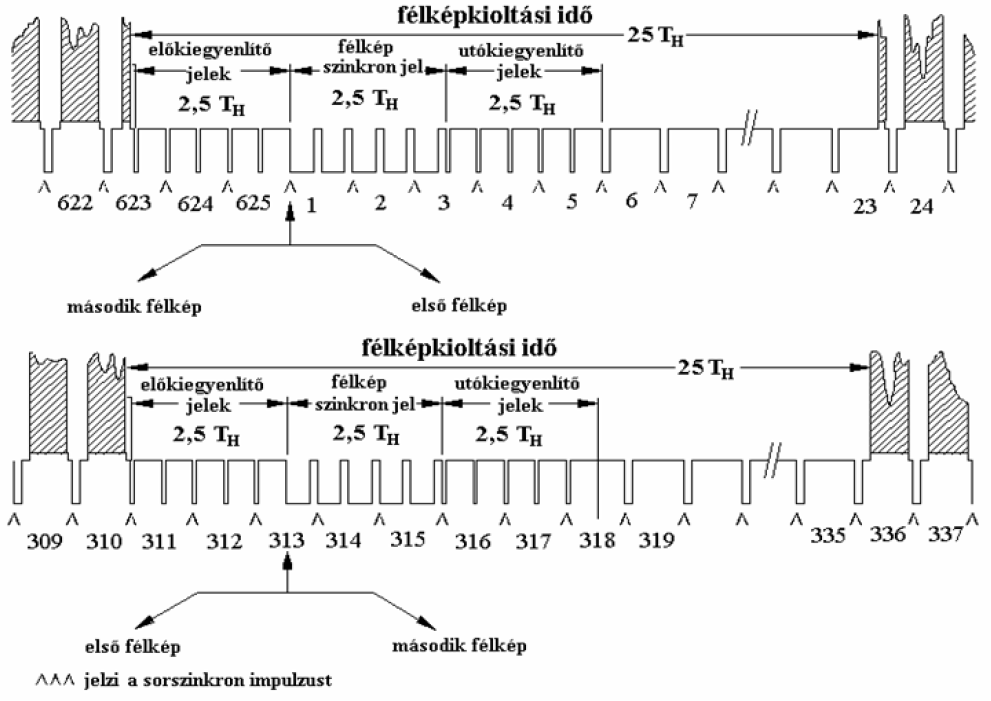
\includegraphics[width= 1\columnwidth  ]{Figures/Vertical_blank_2.png}\\ (a) \\
%    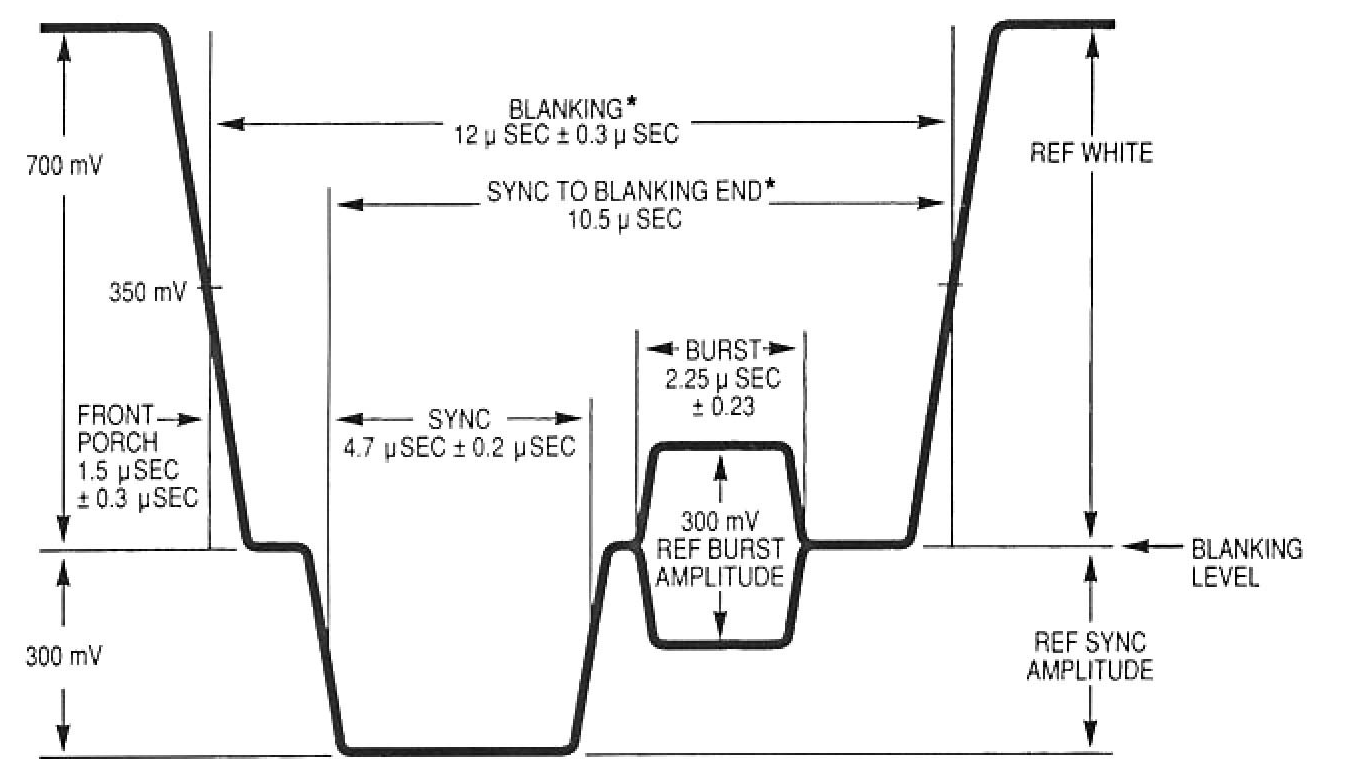
\includegraphics[width= 1\columnwidth  ]{Figures/Horizonta_blank.png}\\ (b) \\
%    \end{minipage} \hfill
%	  \begin{minipage}[c]{0.3\textwidth}
%    \caption{PAL jel félképkioltási intervalluma (a) és sorkioltási intervalluma (b).}
%    \end{minipage}
%\label{fig:PAL}
%\end{figure}

A jelenleg elterjedt megjelenítők esetén ezek a kioltási idők természetesen okafogyottá váltak:
a modern, főként stúdió célú CRT megjelenítők már jóval kisebb kioltási idő mellett is működőképesek, míg LCD megjelenítők esetén egyáltalán nincs szükség kioltási időre.
Ennek ellenére a kioltási idők a jelenlegi digitális szabványok esetén is ugyanúgy jelen vannak, így pl. a HDMI szabvány esetében is.
Ennek egyik, természetes oka az, hogy a technika fejlődésével megjelenő újabb és újabb szabványok mind a már létező, korábbi szabványokra épülnek.
Másrészt a kioltási idők lehetővé tették egyéb, kiegészítő adatok tárolását is ezekben az időszegmensekben.
Így a kioltási időkben továbbítható pl. a teletext adat, feliratok, és digitális esetben a video kísérő audio adat is.
Ezen adatok helyét az ITU-R BT.1364 és az SMPTE 291M szabványok definiálják. 
Megjegyezhető, hogy a szabványok a digitális hang átvitelét (pl. a HDMI szabvány esetén is) a sorkioltási időben írják elő \footnote{
Egy egyszerű példaként HDMI audio átvitelre:
1080p HD formátum esetén (összes sor: 1125, ld. később) $60~\mathrm{Hz}$-es képfrekvencia mellett a sorfrekvencia $f_V = 67.5~\mathrm{kHz}$.
$192~\mathrm{kHz}$ mintavételi frekvenciájú 8 csatornás audioanyag átvitele esetén az egy kép alatt átvivendő audiominták száma: $\frac{8 \cdot 192 000 }{60} = 25600~\mathrm{minta}$, azaz soronként kb. 23 minta átvitele szükséges.
Ez a HDMI 1.0 szabvány által megengedett audiosebesség. (Példa folytatása \href{https://www.sciencedirect.com/science/article/pii/B9780128016305000049}{itt} található.)
}.

% https://www.sciencedirect.com/topics/computer-science/blanking-interval
% https://www.sciencedirect.com/topics/computer-science/horizontal-blanking

\paragraph{Térbeli felbontás és az SD formátum:\\}

Az analóg videojel tárgyalása után a továbbiakban rátérhetünk a videojel digitális reprezentációjának tárgyalására.
Az első digitális videoformátumot a normálfelbontású, SD videót az ITU (akkoriban CCIR) alkotta meg 1982-ben a ITU-601 szabvány formájában \footnote{Munkájáért a CCIR 1983-ban tehcnikai Emmy díjat is kapott}.

Az SD formátum gyakorlatilag az eddig tárgyalt videojel komponensek digitális reprezentációjának tekinthető, azaz a \ref{fig:PAL_frame} látható videojel teljes egészében digitalizációra került kioltási intervallumokkal együtt, mind a luma és chroma komponensekre (más szóval az $Y'P_b'P_r'$ jelek közvetlen digitalizációjával kaphatjuk).
A digitalizált videojelek neve--ahogy arról már szó volt--$Y'C_b'C_r'$ jelek.
A jelek elvi előállítása az \ref{Fig:SD_production} ábrán látható.
\begin{figure}[]
	\centering
	\begin{overpic}[width = 0.8 \columnwidth ]{Figures/YCbCr_production.png}
	\end{overpic}
	\caption{Digitális SD jel előállítása a videokomponensek digitalizálásával}
	\label{Fig:SD_production}
\end{figure}


A digitalizáció egyes kérdéseit már a korábbiakban érintettük.
Nyitott kérdés még a soronkénti mintaszám meghatározása, amely a sorok számával együtt megadja az SD formátum felbontását (pixelszámát).
A feladat tehát az analóg videójel mintavételi frekvenciájának meghatározása.

A mintavételi frekvencia megválasztásánál a következő szempontokat vették figyelembe:
\begin{itemize}
\item Természetes törekvés volt, hogy a több évtizede egymás mellett létező NTSC és PAL rendszerre egyszerre alkalmazható legyen, azaz mind PAL, mind NTSC video digitális ábrázolását lehetővé tegye.
Emellett nyilvánvalóan a mintavételezést úgy kell végrehajtani, hogy mindkét rendszerben egy sorba egész számú mintavételi periódus (azaz pixel) férjen bele.
Ebből következik, hogy a mintavételi frekvencia a sorfrekvencia egész számú többszöröse kell, hogy legyen mind az NTSC, mind a PAL rendszerben, azaz
\begin{equation}
f_s = n \cdot f_H^{\mathrm{PAL}} = m \cdot f_H^{\mathrm{NTSC}},
\end{equation}
ahol $n, m$ egész számok.
Minthogy a sorfrekvenciák 
\begin{align}
f_H^{\mathrm{PAL}} &= 25 \cdot 625 = 15625~\mathrm{Hz} \\
f_H^{\mathrm{NTSC}} &= 30 \cdot \frac{1000}{1001} \cdot 525 = 15734.2~\mathrm{Hz} ,
\end{align}
ezek legkisebb közös többszöröse
\begin{equation}
144 \cdot f_H^{\mathrm{PAL}} = 143 \cdot f_H^{\mathrm{NTSC}} = 2.25~\mathrm{MHz}.
\end{equation}
A mintavételi frekvencia tehát $2.25~\mathrm{MHz}$ egész számú többszöröse.
\item Emellett a mintavételi tétel értelmében a mintavételi frekvencia az átlapolódás elkerülésének érdekében legalább a mintavett jel sávszélességének kétszerese kell, hogy legyen.
Korábban láttuk, hogy a luma jel sávszélessége $6~\mathrm{MHz}$, a chroma jeleké pedig ennek a fele.
\end{itemize}
A legkisebb frekvencia amire a két előbbi feltétel teljesül $13.5~\mathrm{MHz}$.
Ezt választották tehát a világosságjel mintavételi frekvenciájának, miközben a színkülönbségi jelek számára, figyelembe véve az emberi látás tulajdonságait, felezett mintavételi frekvenciát ($6.5~\mathrm{MHz}$) választottak.
Ez az európai rendszerben 1 sorra 864, az amerikaiban 858 teljes mintaszámot eredményez, amely a sorkioltási időt is tartalmazza.

\begin{figure}[]
	\centering
	\begin{overpic}[width = 0.65 \columnwidth ]{Figures/SD_formats.png}
	\end{overpic}
	\caption{Az SD formátum képmérete az amerikai és az európai rendszerben}
	\label{Fig:SD_format}
\end{figure}

A két rendszer további egységesítésének érdekében egy soron belül az aktív pixelek számát közösen 720 pixelre választották (amelyből csak 704 pixel tartalmaz tényleges képi adatot, a digitalizálás előtti analóg jel kezdetének bizonytalansága, szélekhez közeli torzításai, elmosódásai miatt).
Ezzel tehát megkaptuk az SD formátum tényleges képméretét, ahogy az az \ref{Fig:SD_format} ábrán látható.
Az aktív sorok száma alapján, és mivel mindkét rendszerben kizárólag interlaced videó definiált, a két formátum megjelölése \textbf{480i} és \textbf{576i}.
Könnyen belátható, hogy szabványos 4:3 képarány azonos horizontális pixelszám de különböző sorszám mellett csak úgy érhető el, ha az egyes képelemek (pixelek) nem négyzetalakúak (azaz a \textbf{pixel aspect ratio (PAR)} értéke 1-től különböző).
Számítástechnikában a monitorok ezzel szemben négyzetes pixelméretet definiáltak, így az elterjedt számítógépes SD formátum a jól ismert 640x480 pixelszám.
%TODO Pixel apsect ratio, storage aspect ratio, display aspect ratio kifejteni

\begin{figure}[]
	\centering
	\begin{overpic}[width = 0.4 \columnwidth ]{Figures/sd_gamut.png}
	\small
	\put(0,0){(a)}
	\end{overpic}
	\hspace{2mm}
	\begin{overpic}[width = 0.55 \columnwidth ]{Figures/sd_OETF.png}
	\small
	\put(0,0){(b)}
	\end{overpic}
	\caption{Az SD formátum gamutja(a) és Gamma-függvénye (b)}
	\label{Fig:SD_gamut}
\end{figure}

Röviden összefoglalva a jelen, és előző fejezetet a két SD formátum létrehozásának lépései és főbb tulajdonságai:
\begin{itemize}
\item A formátum primary színei és a színtér gamutja a \ref{Fig:SD_gamut} (a) ábrán látható.
A színtér fehérpontja D65 fehér.
A luma komponens számításának módja \footnote{Itt jegyezzük meg, hogy ,,matematikaiatlanul'', ezek a luma együtthatók az NTSC szabvány együtthatókból származnak, tradíció miatt a luma jel számítási módját nem változtatták meg az SD szabvány bevezetésével annak ellenére, hogy az alapszínek megváltoztak. 
Emiatt az $XYZ \rightarrow RGB$ mátrix második sora jelen esetben nem az itt bemutatott luma együtthatókat eredményezné.
Ez egy újabb példa arra, hogy a hasonló matematikai következetlenségek nem állnak távol a gyakorlatban alkalmazott videotechnikától.}
\begin{equation}
Y' = 0.299 R' + 0.587 G' + 0.112 B'
\end{equation}
\item A forrás RGB jelei a perceptuális kvantálás megvalósításának érdekében Gamma-torzításon mennek keresztül, ahol a Gamma-függvény, vagy Optoelectronic Transfer Function:
\begin{equation}
E = 
\begin{cases}
4.500 L, \hspace{20mm} \mathrm{ha}\, L < 0.018 \\
1.099 L^{0.45} - 0.099, \hspace{3mm} \mathrm{ha}\, L \geq 0.018,
\end{cases}
\end{equation}
ahol $L \in \{ R, G, B \}$.
A teljes görbe jól közelíthető egy $L^{0.5}$ függvénnyel
\item A formátum képaránya 4:3. 
A későbbiekben a HD megjelenése után ezt kiegészítették 16:9 képarányú formátummal is.
\item Kizárólag interlaced formátum definiált
\item A videókomponensek megfelelő sávkorlátozás után mintavételezésen és kvantáláson esnek át.
A kvantálás 8, vagy 10 biten történik.
\item A világosságjel mintavételi frekvenciája $f_s = 13.5~\mathrm{MHz}$.
Az 576i (625 soros, 50 félkép/s) rendszerben az aktív felbontás így 720x576 pixel, a 480i (525 soros, 60 félkép/s) rendszerben 720x480 px.
\item A színkülönbségi jel az eredeti, stúdióformátumban 4:2:2, tehát a horizontális színfelbontás a világosságjelének a fele.
Ezt később kiegészítették 4:2:0 struktúrával is konzumer célokra.
\end{itemize}

\section{A HD formátum}

%Whitaker 592. oldal
Az előzőekben részletesen tárgyaltuk as SD digitális videoformátum megalkotásának alapelveit.
A részletes vizsgálat oka, hogy ugyanezek az alapelvek, jelfeldolgozási lépések érvényesek a jelenlegi HD és UHD formátumok esetén is, valamint a jelenlegi SD műsorszórás Magyarországon is 576p (azaz már progresszív) formátumban történik.

Láthattuk, hogy az SD formátum megalkotásánál az egyes paramétereket úgy választották meg, hogy a kitűzött kb. 10 fokos látószögben minél élethűbb képi reprodukciót lehessen megvalósítani.
A HD és UHD formátumok tárgyalása előtt vizsgáljuk meg, hogy adott felbontás (pixelméret) mellett mekkora távolságból kell az adott kijelzőt megfigyelni, rávilágítva ezzel a HD formátum létrehozásának fő motivációjára.

\paragraph{Optimális nézőtávolság:\\}

\begin{figure}[]
	\centering
	\begin{overpic}[width = 0.67 \columnwidth ]{Figures/hd_pixel_angle_mod.png}
	\small
	\end{overpic}
	\caption{Geometria az optimális nézőtávolság származtatásához}
	\label{Fig:optimal_vd}
\end{figure}

Általánosan elmondható, hogy pixel alapú képi reprodukció során a fő szempont, hogy a szomszédos pixelekből érkező fénysugarak által bezárt szög az emberi szem felbontóképessége alá essen.
Ezzel biztosítva van, hogy a kijelző pixelstruktúrája nem látható (a kép nem ,,pixeles''), valamint az RGB alapszíneket alkalmazó reprodukció is lehetővé válik, hiszen az egyes alapszínek érzékelése helyett az additív színkeverés a szemben megvalósul.

Korábban láthattuk, hogy az emberi szem felbontása 1 szögperc (azaz $\frac{1}{60}^{\circ}$) (legalábbis a világosságjelre véve, segítségünkre van, hogy színezetre ennél is rosszabb).
Adott pixelméretre természetesen ebből már meghatározható az a minimális nézőtávolság, amelyre az előbbi feltétel teljesül.
Mivel jellemzően a kijelzőknek nem a pixelmérete van megadva, hanem a kijelző mérete és a vertikális, ill. horizontális pixelszám, ezért célszerű a fenti minimális nézőtávolságot ezek függvényében kifejezni.

Vizsgáljuk az \ref{Fig:optimal_vd} ábrán látható geometriát adott $H$ magasságú, $N_V$ sorszámú kijelző esetén.
A pixelméret ekkor természetesen $\frac{H}{N_V}$.
A kijelző a megfigyelőtől $D$ távolságra helyezkedik el.
A szomszédos (szemközti) pixelekből a megfigyelő szemébe érkező fénysugarakra felírható ekkor a 
\begin{equation}
\tan \frac{\Phi}{2} = \frac{H}{2 N_V D}
\end{equation}
egyenlőség.
Alkalmazzuk a tangens függvény kisargumentumú lineáris közelítését, azaz $\tan x \approx x$, ha $x \ll 1$.
Ekkor
\begin{equation}
\Phi = \frac{H}{N_V D} \hspace{3mm} \rightarrow \hspace{3mm} D = \frac{H}{N_V \Phi}
\end{equation}
érvényes.
Az emberi szem felbontását $\frac{1}{60}\cdot \frac{\pi}{180}~\mathrm{rad} = 2.9 \cdot 10^{-4}$ behelyettesítve adott felbontású és méretű kijelző esetén az optimális (minimális) nézőtávolságra
\begin{equation}
D = H \frac{1}{N_V \,  2.9 \cdot 10^{-4}}
\end{equation}
adódik. 
Ez a távolság az ún. Lechner-távolság, amely tehát megadja, hogy a tervezés során figyelembe vett képméret és felbontás mellett mekkora az optimális nézőtávolság adott képformátum esetén.
\begin{table}[h!]
\caption{Fontosabb SD és HD formátumok ideális nézőtávolsága és az így kitöltött horizontális látószög}
\renewcommand*{\arraystretch}{2.25}
\label{tab:viewing_dist}
\begin{center}
    \begin{tabular}[h!]{ @{}c | | l | l | l @{} }%\toprule
				         &   Amerikai 		   & Európai 				&	 HDTV \\ \hline
    TV-sor/képmagasság:	 &     480 	  		   &   576   				&	 1080\\
    Nézőtávolság:   &  7-szeres képmagasság    &  6-szoros képmagasság & 3-szoros képmagasság \\
    Nézőtávolság:       &  4.25-szörös képátló &  3.6-szoros képátló	& 1.5-szörös képátló \\
    Vízszintes látószög &  kb. 11 fok 		&    kb. 13 fok & kb. 32 fok\\
    \end{tabular}
\end{center}
\end{table}

Amennyiben az $a_r$ képátló ismert (SD esetén 4:3, HD esetén 16:9), az összefüggés kifejezhető a képszélesség függvényében is.
SD esetén ez
\begin{equation}
D = \frac{W}{a_r} \frac{1}{N_V \,2.9 \cdot 10^{-4}},
\end{equation}
ahol $W$ a kép szélessége.
Ekkor ha a kijelzőt az így kapott optimális távolságról nézzük, meghatározható a képernyő által bezárt vízszintes látószög:
\begin{equation}
\tan \frac{\Phi_H}{2} = \frac{W}{2 D} \hspace{1cm} \rightarrow \hspace{1cm} D = \frac{W}{2 \tan \frac{\Phi_H}{2}}, 
\end{equation}
és így adott felbontás mellett a horizontális látószög:
\begin{equation}
\Phi_H = 2\arctan \left( \frac{a_r \, N_V \, 2.9\cdot 10^{-4}}{2} \right).
\end{equation}

Az eredményeket az eddig bemutatott SD és a következőekben tárgyalt HD formátumokra kiszámítva a \ref{tab:viewing_dist} táblázat foglalja össze.
Láthatjuk, hogy az SD felbontást ideálisan a képmagasság 6-7-szereséről célszerű nézni.
Ekkor valóban, a formátum tervezésének kiindulási pontjába érünk vissza, azaz a kijelző a fő látóterünket, kb. 10-13 fokot tölti ki horizontálisan.

Ez már előrevetíti a HD formátum megalkotásának fő célját: a vizuális élmény fokozását nagyobb kitöltött látószög alkalmazásával.
A HD formátum célja tehát---ellentétben a közhiedelemmel---nem a pixelben kifejezett felbontás növelése, és így azonos felületre minél nagyobb számú képpont belezsúfolása, hanem az otthoni vizuális élmény növelése a tartalommal lefedett látótér megnövelésével.

\paragraph{Rövid HD történelem:\\}

A nagyfelbontású (High Definition) formátum létrehozása gyakorlatilag a televíziózás megjelenése óta a teljes XX. századon átívelt.
Noha manapság a kifejezés jellemzően digitális formátumra utal, már a korai analóg technika korában is léteztek HD kezdeményezések.
Olyannyira, hogy már 1949-ben, Franciaországban kísérleti műsorszórást kezdtek monokromatikus (fekete-fehér), de 819 sort alkalmazó analóg rendszerben (a műsorszórás ebben a formátumban egészen 1983-ig tartott).
A Szovjetunióban kísérleti jelleggel 1958-ban kifejlesztettek egy színes, 1125 sorból álló analóg rendszert, a hadászati célra létrehozott technikát azonban végül a gyakorlatban nem hasznosították.
Végül a japán NHK cég vezette be az első mai értelemben vett HD műsorszórást 1989-ben.
Rendszerük, az ún. Hi-Vision, vagy MUSE (Multiple sub-Nyquist Sampling Encoding) 5:3-as képarányú, 1125 soros analóg interlaced videó műsorszórására volt képes.
A japán HD műsorszórás erőteljesen ösztönözte a HD formátum szabványosítását, amely azonban az analóg rendszer hatalmas sávszélességigénye miatt egészen a 90-es évek elejéig nem valósult meg.

A HD szabvány létrejötte végül a digitális tömörítési módszerek, főként az MPEG-1 és MPEG-2 tömörítések megjelenésének köszönhető.
A szabványt 1990-ben tették közre az \href{https://www.itu.int/dms_pubrec/itu-r/rec/bt/R-REC-BT.709-6-201506-I!!PDF-E.pdf}{ITU-709} (Rec. 709) ajánlásban.

\paragraph{HD paraméterek:\\}

Az ITU-709 szabvány a következő HD paramétereket határozta meg:
\begin{itemize}
\item \textbf{Képarány:} az első szabványosított formátumjellemző a HD rendszer képaránya volt, amelyet 16:9 értékűre választottak.
A választás nem kézenfekvő, mivel a formátum létrehozásakor gyakorlatilag nem állt rendelkezésre ebben a képarányban nyersanyag: mind a mozifilmek, mind a korábbi SD formátumú anyagok ettől eltérő képformátumban kerültek rögzítésre.
A korabeli nyersanyagok jellegzetesen 4:3 (SD videó), 15:9, 1.85:1, 2.2:1, illetve 2,35:1 (mozis szabványok) voltak.
Azt találták, hogy amennyiben azonos területű téglalapokat vetítünk egymásra a fenti, gyakori oldalarányokkal, akkor az így kapott téglalap sokaság éppen egy 16:9 oldalarányú téglalapba rajzolható bele.
Továbbá az ezen téglalapok metszete szintén éppen egy 16:9 arányú téglalapot határoz meg.
A geometria a \ref{Fig:kerns_powers} ábrán látható.
\begin{figure}[]
	\centering
	\begin{overpic}[width = 0.9 \columnwidth ]{Figures/KernsPowers.png}
	\small
	\end{overpic}
	\caption{A 16:9 oldalarány, mint sok gyakori képarányú téglalap határoló-síkidoma és metszete}
	\label{Fig:kerns_powers}
\end{figure}
A gondolatmenet eredményeképp, annak érdekében, hogy a legtöbb létező képarányú korabeli nyersanyag optimálisan megjeleníthető legyen az új formátumban esett a választás a ma már jól ismert 16:9 képarányra.

\item \textbf{Képfrissítési frekvencia:} Az SD rendszer hagyatékaként a HD szabvány számos képfrissítési frekvenciát támogat, így a $24~\mathrm{Hz}$, $25~\mathrm{Hz}$, $30~\mathrm{Hz}$, $50~\mathrm{Hz}$ és $60~\mathrm{Hz}$ képfrekvenciákat, valamint és ezek $\frac{1000}{1001}$-szeres módosításait.
Ezen kívül, ezek a frissítési frekvenciák mind progresszív, mind váltottsoros módban alkalmazhatóak.

\item \textbf{Mintavételi frekvencia:}
A mintavételi frekvencia esetében kiindulásul az SD mintavételi frekvencia szolgált.
A HD formátum célja SD-hez képest mind függőleges ($\times 2$), mind vízszintes ($\times 2$) felbontásduplázás, ezen felül a 4:3 képarány helyett 16:9 alkalmazása ($\times 4/3$), amely együttesen a mintaszám--és így a mintavételi frekvencia---legalább $2\times 2 \times \frac{4}{3} = 5.33$-szorozódását jelenti.
A legtöbb képfrekvenciához való kompatibilitás biztosítása érdekében (azaz egy sorba egész számú minta férjen) a mintavételi frekvencia $5.5 \cdot 13.5 = 74.25~\mathrm{MHz}$ lett, illetve törtszámú képfrekvencia esetén ennek az $\frac{1000}{1001}$-szerese.
Progresszív esetben $50-60~\mathrm{Hz}$ képfrekvencia esetén a mintavételi frekvencia ennek a duplája: $fs = 148.5~\mathrm{MHz}$.
%TODO : kibogarászni KovácsI jegyzetéből a mintavételi frek. megválasztását (VidStTech 01.pdf, 46.o)
\item \textbf{Felbontás:} Hosszas egyeztetések után\footnote{Az első HD szabvány a Japán rendszer nyomán 1035 sort definiált. Ezt később visszavonták} a szabvány 1080 aktív sort definiált 1125 teljes sorszámmal mind progresszív, mind váltottsoros letapogatás mellett (SMPTE 274M szabvány).
Emellett a különböző képfrekvenciák egységes kezelése érdekében a soronkénti mintaszámot fixen 1920 mintára választották, így a HD formátum felbontása 1920x1080 pixel.
A különböző képfrekvenciájú HD formátumok így tehát kizárólag a soronkénti inaktív pixelek számában különböznek egymástól (azaz a sorkioltási idő hosszában).

\begin{table}[h!]
\caption{Néhány HD formátum mintavételi frekvenciája, összes sor és oszlopszáma, felbontása. 
A soronkénti pixelek száma $S_{\mathrm{LT}} = $} alapján számítható.
\renewcommand*{\arraystretch}{2.25}
\label{tab:viewing_dist}
\begin{center}
    \begin{tabular}[h!]{ @{}c | l | l | l | l | l @{} }%\toprule
		Rendszer     &   $f_s \, [\mathrm{MHz}]$ 				& $S_{TL}$ & $L_T$ & Aktív pixelszám \\ \hline
		$720p50$     &   $74.25~\mathrm{MHz}$    				& 1980     &  750  & $1280 \times 720$ \\
		$720p59.94$  &$74.25\cdot\frac{1000}{1001}~\mathrm{MHz}$& 1650     &  750  & $1280 \times 720$ \\
		$1080i25$ 	 &   $74.25~\mathrm{MHz}$    				& 2640     & 1125  & $1920 \times 1080$ \\
		$1080i30$  	 &   $74.25~\mathrm{MHz}$    				& 2200     & 1125  & $1920 \times 1080$ \\
		$1080p50$ 	 &   $148.5~\mathrm{MHz}$    		    	& 2640     & 1125  & $1920 \times 1080$ \\
		$1080p59.94$ &$148.5\cdot\frac{1000}{1001}~\mathrm{MHz}$& 2200     & 1125  & $1920 \times 1080$ 
        \end{tabular}
\end{center}
\end{table}

A különböző HD formátumok jelölése a következő:
\begin{itemize}
\item Teljes aktív felbontás pixelben kifejezve.
Gyakran rövidítésképp csak a vertikális méretet jelölik meg.
\item képletapogatás módja: $p$ a progresszív, $i$ az interlaced letapogatást jelöli
\item képfrekvencia (frame rate) mind $p$, mind $i$ esetben.
Interlaced videó esetén gyakran a képfrekvencia helyett---hibásan---a félképfrekvenciát jelölik.
\end{itemize}
Így pl. az $1080i25$ a 1080 soros, váltottsoros $25~\mathrm{Hz}$ képfrekvenciájú, és $50~\mathrm{Hz}$ félkép-frekvenciájú formátumot jelöli.
\begin{figure}[]
	\centering
	\begin{overpic}[width = 1 \columnwidth ]{Figures/HD_format.png}
	\small
	\end{overpic}
	\caption{Az 1080 soros és 720 soros HD formátum szemléltetése}
	\label{Fig:HD_formats}
\end{figure}

A progresszív HD formátumok nagy adatsebesség-igénye miatt az ITU-709-et néhány évvel később kibővítették egy alacsonyabb felbontású formátummal, ez 720 aktív sort és 1280 aktív pixelt alkalmaz, és kizárólag progresszív letapogatással definiálták \footnote{Az 1080p bevezetése során az egyik kitűzött cél a legalább duplázott sorszám volt.
A 720p az SD és HD között félúton: másfélszeres sort alkalmaz így a sorszáma $\frac{3}{2} \cdot 480 = 720$-ból adódik, míg az oszlopszám a 16:9 képarányból, négyzetes pixelek mellett}.
Jelölése: \textbf{720p}.
A két HD formátumra egy-egy példa a \ref{Fig:HD_formats} ábrán látható.
\item A HD formátum alapszínei az SD ITU-601-el megegyezőek, így a gamutja is azonos.
A luma komponens számításának módja 
\begin{equation}
Y' = 0.2126 R' + 0.7152 G' + 0.0722B'.
\end{equation}
\begin{figure}[]
	\centering
	\begin{overpic}[width = 1\columnwidth ]{Figures/hd_line.png}
	\end{overpic} 
	\caption{1080 soros HD formátum egy sorának felépítése}
	\label{Fig:hd_line}
\end{figure}
Az együtthatók az SD-vel ellentétben már kolorimetriailag is helyesek, azaz a színtér alapszíneiből (és fehérpontjából) felírható $RGB \hspace{3mm} \rightarrow \hspace{3mm} XYZ$ transzformációs mátrix $Y$ sorából ugyanezeket a világosság-együtthatókat kapnánk.
\item A szabvány Gamma-karakterisztikája az SD-vel megegyező:
\begin{equation}
E = 
\begin{cases}
4.500 L, \hspace{20mm} \mathrm{ha}\, L < 0.018 \\
1.099 L^{0.45} - 0.099, \hspace{3mm} \mathrm{ha}\, L \geq 0.018,
\end{cases}
\end{equation}
ahol $L \in \{ R, G, B \}$.
\item A szabvány az SD-vel azonos 8 és 10 bites digitális reprezentációt ír elő.
\item A stúdió szabvány alapvetően 4:2:2 szín-mintavételezési struktúrát definiál.
\end{itemize}
A szabványos HD videójel ezek mellett teljesen az SD-vel azonos felépítésű, egy egyszerű példa a \ref{Fig:hd_line} ábrán látható.
Az egyetlen különbség gyakorlati megvalósítás szempontjából, hogy a kioltási időszakokban a szinkron impulzusok ún. 3 állapotúak ($0, \pm300~\mathrm{mV}$).

\paragraph{Tömörítetlen videó adatsebesség:\\}

Vizsgáljuk most néhány alapvető képformátum esetén a videó tömörítetlen adatsebességét!
Az aktív és teljes pixelszámokat a \ref{Fig:size} ábrán látható jelölésekkel jelölve a teljes adatsebesség
\begin{equation}
B\!R_T = \underbrace{S_{TL} \cdot L_T \cdot f_f \cdot n_{\mathrm{bit}}}_{\text{mintánkénti bitrate}} \cdot n_{\mathrm{CS}},
\end{equation}
ahol $f_f$ a képfrekvencia, $n_{\mathrm{bit}}$ a mintánkénti bitszám és $n_{\mathrm{CS}}$ a színkülönbségi jelek alulmintavételezését jelöli (komponens/minta).
Utóbbi értéke 4:4:4 struktúra esetén $n_{\mathrm{CS}} = 3$, 4:2:2 estén $n_{\mathrm{CS}}=2$, 4:2:0 esetén $n_{\mathrm{CS}} = 1.5$.

Hasonlóan, az aktív tartalom bitsebessége
\begin{equation}
B\!R_A = S_{TA} \cdot L_A \cdot f_f \cdot n_{\mathrm{bit}} \cdot n_{\mathrm{CS}}
\end{equation}
alapján számítható.

Néhány gyakran alkalmazott videóformátum teljes és aktív videósebessége a \ref{tab:bitrate} táblázatban látható\footnote{Az UHD formátum kioltási idejei \href{http://programmersought.com/article/7908103552/}{szabványosan} 90 inaktív sor és 560 inaktív pixel/sor}.
\begin{figure}[]
\captionsetup{singlelinecheck=off}
	\centering
	\begin{minipage}[c]{0.4\textwidth}
	\begin{overpic}[width = 1\columnwidth ]{Figures/size.png}
	\end{overpic}   \end{minipage}\hfill
		\begin{minipage}[c]{0.55\textwidth}
	\caption[]{Jelölés-konvenció az adatsebesség számításához
	\begin{itemize}
	\item $S_{TL}$: Összes mintaszám/sor
	\item $S_{TA}$: Aktív mintaszám/sor
	\item $L_T$: Összes sor/kép
	\item $L_A$: Aktív sor/kép
	\end{itemize}}
	\label{Fig:size}  \end{minipage}
\end{figure}
%
\begin{table}[h!]
\caption{Videóformátum mintavételi frekvenciája, összes sor és oszlopszáma, felbontása, $n_{\mathrm{bit}} = 10$ bitmélység esetén}
\renewcommand*{\arraystretch}{2.25}
\label{tab:bitratet}
\begin{center}
    \begin{tabular}[h!]{ @{}c | l | l | l | l | l @{} }%\toprule
\thead{Rendszer} & \thead{Mintavételi \\ frekvencia} &    \thead{Teljes bitrate \\ 4:2:2} & \thead{Aktív bitrate\\ 4:2:2} & \thead{Aktív bitrate\\ 4:4:4} \\ \hline
$576p50$     &   $13.5~\mathrm{MHz}$        & $0.54~\mathrm{Gbit/s}$  & $0.41~\mathrm{Gbit/s}$ & $0.62~\mathrm{Gbit/s}$ \\
$720p60$     &   $74.25~\mathrm{MHz}$    	& $1.49~\mathrm{Gbit/s}$  & $1.11~\mathrm{Gbit/s}$ & $1.67~\mathrm{Gbit/s}$ \\
$1080i30$ 	 &   $74.25~\mathrm{MHz}$    	& $1.49~\mathrm{Gbit/s}$  & $1.24~\mathrm{Gbit/s}$ & $1.86~\mathrm{Gbit/s}$ \\
$1080p60$ 	 &   $148.5~\mathrm{MHz}$    	& $2.97~\mathrm{Gbit/s}$  & $2.49~\mathrm{Gbit/s}$ & $3.73~\mathrm{Gbit/s}$ \\
$2160p60$ 	 &   $297~\mathrm{MHz}$         &  $11.88~\mathrm{Gbit/s}$& $9.96~\mathrm{Gbit/s}$ & $14.93~\mathrm{Gbit/s}$
\end{tabular}
\end{center}
\end{table}
%
Látható, hogy a $720p$ és $1080i$ formátumok tömörítetlenül azonos adatmennyiséget generálnak, ugyanakkor nagy előnye a progresszív formátumnak jóval hatékonyabban tömöríthetősége.
Ahogy korábban a váltott-soros formátum előnye ezzel szemben, hogy állóképekre a progresszívvel azonos vertikális felbontást biztosít, bár gyors mozgásokra ez a felbontás romlik.
Épp ezért, azon műsorszolgáltatók, amelyeknél a sport-tartalom elsődleges jellemzően a $720p50/60$ formátumot használ, míg a főként filmeket, hírműsorokat sugárzó operátorok jellemzően $1080i$-t alkalmaznak.
Magyarországon jelenleg a HD adások mellett minden szolgálgató biztosít SD felbontású verziót is, amely jellemzően $576p50$ formátumot alkalmaz.

Jelenleg stúdiótechnikában a legelterjedtebb digitális videóinterface az SDI (Serial Digital Interface), konzumer elektronikában pedig a HDMI (High-Definition Multimedia Interface).
A fenti adatsebességek kézzelfoghatóvá-tételéhez, néhány jelenleg is használt HDMI verzió a következő adatmennyiségek továbbítását teszi lehetővé:
\begin{itemize}
\item HDMI 1.0-1.2: 4.95 Gbit/s (3.96 Gbit/s tényleges)\footnote{A HDMI szabvány itt nem részletezett okokból ún. 8b/10b csatornakódolást alkalmaz, amely során 8 bitnyi adatot 10 biten visz át.
A 4.95 Gbit/s teljes sávszélességnek tehát csak $\frac{8}{10}$ része használható ki tényleges adatra.}
\item HDMI 2.0: 18 Gbit/s (14.4 Gbit/s tényleges)
\item HDMI 2.1: 48 Gbit/s (38.4 Gbit/s tényleges)
\end{itemize}
Természetesen a HDMI méretezéshez a fenti táblázatból a teljes adatsebességet kell tekinteni, hiszen a HDMI kábelen terjedő HD jel tartalmazza a kioltási időket is: mint korábban tárgyaltuk ezekben az időrésekben kerülnek az audio csatornák és egyéb járulékos adatok elhelyezésre.
Látható, hogy a HDMI 1.0 szabványt főként 1080p videó továbbítására fejlesztették ki 4:2:2 formátum 10, vagy 12 bit, míg 4:4:4 formátum már csak 8 biten továbbítható.
A HDMI 2.0 szabványt már 4k míg a 2.1 szabvány 8k UHD videó továbbítására fejlesztették ki.

%TODO 8b/10b codin
% Fischer Digital Video and Audio broadcasting technology 227.o

%TODO HD ready
%TODO Gaumt coverage percentage, Surface colors
%TODO In typical production practice the encoding function of image sources is adjusted so that the final picture has the desired aesthetic look, as viewed on a reference monitor with a gamma of 2.4 (per ITU-R BT.1886) in a dim reference viewing environment (per ITU-R BT.2035).[10][11][12]
%TODO Rec. 2100, a standard for HDTV and UHDTV with high dynamic range

\section{Az UHD formátum}

Láthattuk, hogy a HD formátum megalkotása során a fő cél a néző látóterének---az SD-hez képest---nagyobb részének tartalommal való kitöltése volt.
A HD-hez hasonlóan az UHD (Ultra High Definition) formátum a vizuális élmény továbbfokozását tűzte ki fő céljául a pixel-szám---és így a kitöltött látószög---további növelésével.

Hasonlóan a HD-hoz, a továbbemelt felbontású formátum fejlesztése a japán NHK nevéhez kötődik, akik már 2003-ban kísérleti UHDTV felvételt készítettek 16 darab HDTV rögzítővel és 4 darab 3840x2048 felbontású CCD szenzorral.
Az első UHDTV szabvány ezek után már 2007-ben megjelent (SMPTE 2036), majd a jelenleg is érvényben lévő \textbf{ITU-R BT.2020} szabványt 2012-ben fogadták.
A szabvány két új formátum paramétereit kodifikálja, a 4k formátumot, amely az 1080 soros HD formátumhoz képest mindkét dimenzió mentén duplázott felbontást (így 4-szeres teljes pixelszámot) alkalmaz, és a 8k-t, amely a 4k-hoz képest kétszeres felbontást definiál.
\begin{figure}[]
	\centering
	\begin{overpic}[width = 0.85 \columnwidth ]{Figures/fov_formats.png}
	\small
	\end{overpic}
	\caption{Az egyes formátumok által biztosított horizontális látószög, a kijelzőt ideális nézőtávolságból nézve.}
	\label{Fig:fov_formats}
\end{figure}

A szabvány célja szerint ideálisan a 4k formátum a néző horizontális látószögéből kb. $58^{\circ}$-ot, a 8k formátum $96^{\circ}$-ot tölt ki, azaz már a periférikus látás jelentős részét is tartalommal tölti ki.
Az egyes formátumok által ideálisan kitöltött látószög változását a \ref{Fig:fov_formats} ábra szemlélteti.

Ahhoz, hogy az ekkora látószögben megfelelő minőségű képi reprodukció valósuljon meg, az ITU-2020 szabvány számos szempontból javította a HD formátum alapparamétereit:
\begin{itemize}
\item \textbf{Felbontás: } A szabvány két felbontást deifiniál, ezek a 3840x2160 (4k) és a 7680x4320 (8k) aktív képméretek.
A HD szabványnak megfelelően mindkét formátum képaránya 16:9 és négyzetes pixelekből áll.
\item A HD-vel ellentétben az ITU-2020 szabvány már kizárólag csak progresszív letapogatást támogat (így a $p/i$ formátummegjelölés UHD esetén okafogyott.
Fontos, hogy a kijelző már optimális esetben a néző periférikus látásának jelentős részét is kitölti, ahol az érzékelést már a szem pálcikái dominálják.
Mivel ezek fúziós frekvenciája jóval nagyobb, mint a fő látóterünké, ezért a villogás elkerülése érdekében a képfrekvenciát az UHD esetében emelni kellett.
Ennek megfelelően a szabvány a 120, 119.88, 100, 60, 59.94, 50, 30, 29.97, 25, 24, 23.976 Hz képfrekvenciákat támogatja.
\begin{figure}[]
	\centering
	\begin{overpic}[width = 0.75 \columnwidth ]{Figures/uhd_gamut.png}
	\small
	\end{overpic}
	\caption{Az ITU-2020 szabvány gamutja, összehasonlítva a HD színtérrel}
	\label{Fig:UHD_gamut}
\end{figure}

\item \textbf{Színtér:} Az ITU-2020 szabvány az NTSC óta először új alapszíneket vezetett be a nagyobb ábrázolható színtartomány érdekében (és a világosság dinamikatartományának növelése érdekében, ld. köv. pont).
A szabvány színterének gamutja a \ref{Fig:UHD_gamut} ábrán látható.
Megfigyelhető, hogy a választott alapszínek spektrálszínek (azaz a színpatkó határán helyezkednek el), az RGB hullámhosszok rendre 630 nm, 532 nm és 467 nm
\footnote{Természetesen ez nem azt jelenti, hogy az UHD kijelzők RGB fényforrásai spektrálszínek lennének, a szabvány csak a tároláshoz és továbbításhoz használt színteret kodifikálja. 
A megjelenítés már az egyes kijelzők saját színterében történik, amit a ténylegesen alkalmazott alapszínek korlátoznak.
Szakmai körökön belül napjainkban is fontos hírnek számít, ha egy kijelző az ITU-2020 szabványos színterét közel egészében képes megjeleníteni.
Így pl. 2018-ban a JDI cég \href{https://www.displaydaily.com/?view=article&id=62235:jdi-may-have-commercial-problems-but-has-technical-highlights}{bemutatott} egy 17.3"-es kijelzőt, amely lézeres háttérvilágítással az ITU-2020-as szabvány gamutjának 97\%-át képes megjeleníteni.}.
Ezzel a CIE színpatkó 75.8\%-át lefedi (összehasonlításképp, a HD esetében ez 35.9\%), és a Pointer féle valós felületi színek egészét\footnote{
A Pointer féle valós felületi színek azon színek halmaza, amelyek a természetben előfordulnak, mint valamely felületről visszavert fény által keltett színérzet (ellentétben a természetben elő nem forduló színekkel, pl. neon, vagy monitor által kikevert színek).
A Pointer gamutot egy 4089 mintából álló mérési adatbázisból állították össze, és publikálták az eredményeket 1980-ban, azóta a Pointer gamut-lefedés az egyes színterek minősítésének de facto szabványa.
A Pointer féle gamut \href{https://cinepedia.com/picture/color-gamut/}{itt} található, illetve \href{https://www.tftcentral.co.uk/articles/pointers_gamut.htm}{itt} található egy összehasonlítás a gyakran alkalmazott színterek gamutjával.
}.
Az új alapszínekből a világosság a következőképp számítható:
\begin{equation}
Y = 0.2627 \, R + 0.6780 \, G + 0.0593 \, B.
\label{eq:2020_Y}
\end{equation}
\item \textbf{Mintánkénti bitszám:} A tárolt színek tartományának növelése természetesen magával vonja a világosságjel dinamikatartományának növekedését is (nyilván, hiszen adott szín világosságtartalma \ref{eq:2020_Y} alapján az RGB értékekből kiszámítható).
UHD esetében  tehát már nem csak az SD esetében ökölszabályként tárgyalt 100:1 dinamikatartomány ábrázolása volt a cél.
Ennek oka, hogy a 100:1 dinamikatartomány a látás fő látóterében, rögzített tekintet mellett értelmezendő.
Amennyiben egy jeleneten belül a nézőnek lehetősége van körülnézni, úgy a pupilla tágulása és összeszűkülése ezt a dinamikatartományt kb. 5-szörösére emeli.
Mivel rendeltetésszerűen egy UHD kijelző akkora részét tölti ki a látómezőnek, hogy ez a lokális adaptációs mechanizmus végbe tud menni, így a megfelelő reprodukált dinamikatartomány biztosításához a reprezentálandó dinamikatartományt is növelni kellett.
Részben ezt valósítja meg a szabvány növelt gamutja, illetve erre szolgál a jelenleg elterjedőben levő HDR kiegészítés is.
Az ábrázolt dinamikatartomány növelése természetesen magával vonja az ábrázolásra használt bitek számának növelését is, hogy az egyes szintekhez tartozó világosságértékek közti különbség továbbra is az emberi látás modulációs küszöbje alatt maradjon.
Kísérletek kimutatták, hogy a  ITU-2020 színterének perceptuális kvantálásához 11 bit elegendő, így a szabvány a HD szabvánnyal ellentétben már kizárólag 10 és 12 bit reprezentációt ír elő.
\item \textbf{Gamma függvény:} Az ITU-2020 szabvány Gamma-korrekciós függvénye az SD és HD szabványokkal megegyezik:
\begin{equation}
E = 
\begin{cases}
4.500 L, \hspace{20mm} \mathrm{ha}\, L < \beta \\
\alpha L^{0.45} - (\alpha - 1 ), \hspace{3mm} \mathrm{ha}\, L \geq \beta,
\end{cases}
\end{equation}
ahol $\alpha = 1.09929682680944$ és $\beta = 0.018053968510807$.
Különbségként látható: a szabvány a függvény paramétereit nagyobb pontossággal definiálja, és 12 bites ábrázolás esetén a paraméterek 5 tizedesjegy pontossággal számolandók.
\item \textbf{Mintavételi struktúra:} A szabvány 4:2:0, 4:2:2 és 4:4:4 chromamintavételi-struktúrákat engedélyez, utóbbi esetben természetesen luma/chroma jelek helyett közvetlenül RGB jelek kerülnek tárolásra és átvitelre.
4:2:0 és 4:2:2 esetében az $YC_bC_r$ ábrázolás mellett lehetőség van ún. konstans fénysűrűségű luma-chroma reprezentációra is.
\end{itemize}

%TODO \paragraph{Konstans fénysűrűségű mód:\\}
\begin{figure}[]
	\centering
	\begin{overpic}[width = 0.75 \columnwidth ]{Figures/optimal-viewing-distance-television-graph-size.png}
	\small
	\end{overpic}
	\caption{Optimális nézőtávolság a kijelzőátmérő függvényében}
	\label{Fig:optimal_vd_2}
\end{figure}

A fejezet zárógondolataként térjünk vissza a különböző sorszámú kijelzők ideális nézőtávolságához, az ún. Lechner távolsághoz.
Az optimális nézőtávolságra vonatkozóan számos ajánlás létezik, így léteznek gyártói, forgalmazói, illetve THX ajánlások.
\begin{itemize}
\item SMPTE 30: a már tárgyalt, Lechner távolságon alapuló ajánlás, amely HD felbontás esetén 1.6 x képátló nézőtávolságot ír elő, így a horizontális látószög kb. 30 fok.
Ez a házimozi közösségen belül legelfogadottabb, általános nézőtávolság
\item Gyártói és forgalmazói ajánlás: HD felbontás esetén 2.5 x képátló nézőtávolság, így a horizontális látószög kb. 20 fok.
\item THX ajánlás: HD felbontás esetén 1.2 x képátló nézőtávolság, így a horizontális látószög kb. 40 fok, amely a THX szerint a legjobban közelíti a mozikban biztosított élményt.
\end{itemize}
Bár a fenti ajánlások jelentősen eltérnek egymástól, abban azonban egyetértenek, hogy "minél közelebb, annál jobb".

Az optimális nézőtávolság ábrázolható a képernyőátmérő függvényében különböző videóformátumok mellett.
Az így kapott grafikont \ref{Fig:optimal_vd_2} mutatja.
Ekkor egy adott képernyő méret mellett a nézőtávolságot növelve természetesen a pixelstruktúra nem válik láthatóvá, így pl. az $1080p$ vonala fölött a HD kijelzők használhatók.
A gondolatmenet alapján a grafikon területekre oszthatók, amelyek megadják, egy adott kijelzőméret és nézőtávolság mellett milyen felbontású kijelző az optimális választás.

Statisztikák szerint (egy szintén Bernard J. Lechner nevéhez köthető felmérés szerint) a háztartásokban az átlagos nézőtávolság kb. 2.7 méterre adódott.
Ekkora nézőtávolság mellett 50" képátló felett már 1080p felbontású TV-t érdemes venni, míg az UHD tartalom adta előnyök kiélvezéséhez legalább 75"-es ($\sim 1.9~\mathrm{m}$) kijelzőre lenne szükség.
Jelenleg az ekkora kijelzők természetesen még nem elterjedtek, így ez az adat leginkább azt mutatja, hogy jelenleg a 4k tartalmak előnyeit sem használják ki teljes egészében a kijelzők, és a vásárlók nagyrésze.
Ennek ellenére mára sorra jelennek meg a konzumer felhasználásra szánt 8k felbontású kijelzők is, és a 8k műsorszórás is kísérleti jelleggel megkezdődött.
Többek között 2017-ben lőtték fel az első dedikáltan 8k tartalom közvetítésére szánt műholdat (BSAT-4a), amely tervek szerint a 2020-as Japánban tartandó nyári olimpiát hivatott 8k felbontással az ITU-2020 szabvány szerint közvetíteni (amelyet végül a koronavírus járvány miatt 2021 nyarára ütemeztek át).


%Periférikus látás:
%https://www.quora.com/What-is-the-aspect-ratio-of-human-vision

%TODO \subsection{A HDR kiterjesztés}

\vspace{2cm}
\noindent\rule{12cm}{0.4pt}

\subsection*{Ellenőrző kérdések}

\begin{itemize}
\item Mi volt az oka a váltottsoros formátum bevezetésének?
Mi volt a váltottsoros megoldás lényege?
\item Mik voltak az SD formátum mintavételi frekvenciájának szempontjai?
Hogy következett ebből a HD formátum mintavételi frekvenciája?
\item Határozza meg egy 65" átmérőjű 2160p kijelző (16:9 képarányú) ideális nézőtávolságát!
\item Sorolja fel az UHD szabvány néhány újdonságát az SD-hez és HD-hez képest!
\item Határozza meg $2160p60$ formátum esetén az aktív és teljes pixelszámot! 
Az inaktív sorok száma a szabvány szerint 90 sor.
A mintavételi frekvencia $297~\mathrm{MHz}$.
\item Határozza meg az előző feladat formátumára a teljes adatsebességet 4:2:2 mintavételi struktúra esetén, 12 bit/minta ábrázolás mellett!
Hányas HDMI verzió képes a videóadat továbbítására, ha a HDMI interface szabványosan 8 bitnyi adatot 10 biten ábrázol és visz át, és a különböző verziók sebességei a következők:
\begin{itemize}
\item HDMI 1.0-1.2: $4.95~\mathrm{Gbit/s}$
\item HDMI 1.3-1.4: $10.2~\mathrm{Gbit/s}$
\item HDMI 2.0-1.2: $18~\mathrm{Gbit/s}$
\item HDMI 2.1: $48~\mathrm{Gbit/s}$
\end{itemize}
\end{itemize}